%Resume protokol
%kelompok 3 D4 TI-2B 
%Fikri aldi nugraha                  1164038
%Nur Arkhamia Batubara               1164049 
%Miftahul Hasanah                    1164046 
%Si Made Angga Dwitya P              1164053 
%Widary Anggraini Mindo V Siahaan    1164057

\documentclass{article}

\title{PROTOCOL}
\author{}
\date{}

\begin{document}

\maketitle

\section{Pengenalan Protokol} 

Dalam jaringan computer, protocol merupakan konvensi yang disepakati untuk komunikasi antarkomputer. Selanjutnya, protocol TCP/IP 
mendefinisikan bagaimana pesan dikirimkan melalui internet, sedangkan protocol FTP, yang dibangun menggunakan protocol TCP/IP, 
mendefinisikan pesan-pesan FTP dikirim dan diterima. Dan dalam sistem jaringan dan komunikasi, ada spesifikasi prosedur yang diikuti 
saat akan mengirim atau menerima data. Protocol menentukan format, waktu, urutan, dan system pengecekan kesalahan yang digunakan.

Apabila dua buah system yang saling berkomunikasi, hal pertama yang dibutuhkan adalah kesamaan bahasa yang digunakan. Sehingga dapat 
memahami alur proses komunikasi. Lain halnya apabila dua buah system saling berkomunukasi dengan bahasa yang berlainan, tentunya dua 
system tersebut tidak akan saling memahami. Untuk itu, system tersebut membutuhkan sebuah mekanisme pengaturan bahasa yang dapat 
dipahami oleh dua buah system tersebut sehingga pertukaran informasi antar system akan dapat terjadi dengan benar. Aturan bahasa 
komunikasi ini sering disebut protocol komunikasi. 
 
Suatu standar pertukaran informasi. Komputer dengan system operasi dan software berbeda dapat saling berkomunikasi melalui internet 
karena pengadopsian protokol. Seperangkat aturan umum (atau bahasa) yang mengijinkan komputer-komputer untuk saling berkomunikasi. 
Protokol yang standart adalah TCP/IP (Transmission Control Protocol/Internet Protocol). Web menggunakan server protokol HTTP agar 
komputer dapat mengakses file , melakukan pencetakan, berkomunikasi, dan menyediakan layanan lain bagi user lain dalam jaringan.
 
 \ref{layer} 
    \begin{figure}[ht] 
    \centerline{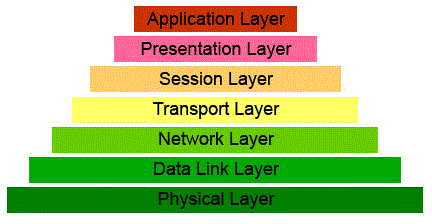
\includegraphics[width=1\textwidth]{figures/layer.JPG}} 
    \caption{osi layer.} 
    \label{layer} 
    \end{figure}
    
 Seperangkat aturan formal yang mendeskripsikan bagaimana cara mentransfer data, terutama dalam jaringan. Protocol level bawah
 mengobservasi standar elektrikal dan fisikal, perintah bit dan byte, pendeteksian transmisi dan kesalahan, serta koreksi terhadap 
 aliran bit. Protocol level atas berkaitan dengan pemformatan data, meliputi sintax pesan, terminal dari dialog computer, susunan 
 karakter, urutan pesan, dan lain-lain.
 
 Ketika data ditransmisikan diantara dua atau lebih peralatan, diperlukan sesuatu yang dapat menjaga control agar data tetap utuh, yaitu 
 suatu deskripsi formal mengenai pesan dan aturan yang harus diikuti oleh dua computer yang ingin bertukar pesan. Protocol dapat 
 mendeskripsikan detal dari interface mesin ke mesin level bawah (cara bagaimana dua program mentransfer file melalui internet).
 
 \section{Elemen Penting Protokol}
 \begin{enumerate}
 \item  Syntax, mengacu pada struktur atau format data, yang mana dalam urutan tampilannya memiliki makna tersendiri.
 \item  Semantics, mengacu pada maksud setiap section bit. Dengan kata lain adalah bagaimana bit-bit tersebut terpola untuk dapat 
 diterjemahkan.
 \item  Timing, mengacu pada 2 karakteristik, yakni kapan data harus dikirm dan seberapa cepat data tersebut dikirim.
 \end{enumerate}

 
 \section{Pengertian Protokol}
Protokol merupakan aturan dalam melakukan pengiriman data (berupa blok-blok data) dari sebuah node jaringan ke node jaringan lain.
Protokol merupakan sarana komunikasi antara mesin melalui jaringan yang terstandarisasi. Protokol mengizinkan data untuk ambil bagian 
dalam transmisi kilat, kemudian ditransmisikan, lalu dikumpulkan kembali sesuai arah dengan perintah yang benar. 
Protokol digunakan untuk mendeteksi kesalahan, tipe kompresi, dan bagaimana receiver (penerima) mengindikasikan bahwa pesan telah 
diterima. 
Protokol dapat mendeskripsikan detail level bawah dari interface machine to machine atau pertukaran level atas antara program alokasi. 
Protokol level bawah meliputi observasi terhadap standar elektrik dan fisik, perintah bit dan byte, pendeteksian transmisi dan 
kesalahan, dan koreksi aliran bit. 
Protokol level atas berkaitan dengan pemformatan data, meliputi sintaks pesan, dialog dari terminal ke komputer, dan pengurutan pesan. 

Protocol merupakan seperangkat aturan komunikasi dimana dalam sebuah hubungan telekomunikasi dapat digunakan untuk menerima sinyal. 
Dalam  koneksi telekomunikasi tersebut protocol dapat  koita bagi menjadi 7 level. Salah satunya yaitu hardware protocol telepon dan 
berupa end point dalam sebuah program komunikasi dalam computer yang sama atau memiliki lokasi yang berbeda-beda. Jadi kedua end point 
tersebut harus dapat mengenali satu sama lain dan mengobservasi protocol.

 \section{Jenis-Jenis Protokol}
Protokol jaringan adalah berbagai protokol yang terdapat dari lapisan  teratas sampai terbawah yang ada dalam sederetan protocol.
Di pandang dari sudut komunikasi data,ada beberapa protokol yang banyak digunakan pada jaringan computer, di antaranya:

 \subsection{TCP/IP}
TCP/IP merupakan protokol standar pada jaringan internet yang tidak tergantung pada jenis computer yang digunakan.
Barangkali perlu dicatat bahwa TCP/IP adalah perlengkapan standar pada sistem operasi Unix dan turunannya.
Saat ini mesin novell,SUN maupun Machintosh sudah dilengkapi protokol standar TCP/IP ini.

Protocol adalah spesifikasi forma yang mendefenisikan prosedur-prosedur yang harus diikuti ketika mengirim dan menerima data (Wermer, 
1996). Protocol mendefenisikan jenis, waktu, urutan dan pengecekan kesalahan yang digunakan dalam jaringan. Transmission control 
protocol/internet protocol (TCP/IP) merupakan protocol untuk mengirim data antar computer pada jaringan. Protocol ini merupakan protocol 
yang digunakan untuk akses internet dan digunakan untuk komunikasi lobal. TCP/IP terdiri atas dua protocol yang terpisah. TCP/IP 
menggunakan pendekatan lapisan (layer) pada saat membangun protocol ini. Dengan adanya pendekatan berlapis ini memungkinkan dibangunnya 
beberaa layanan kecil untuk tugas-tugas khusus.

TCP/IP terdiri dari lima layer, yaitu :
\begin{enumerate}
\item   Layer Application, di dalam layer ini aplikasi seperti FTP, Telnet, SMTP, dan NFS dilaksanakan.
\item   Layer Transport, di dalam layer ini TCP dan UDP menambah data transport ke paket dan melewatkannya ke layer Internet.
\item    Layer Internet, Layer ini mengambil paket dari layer transport dan menambahkah informasi alamat sebelum mengirimkankannya ke layer network interface.
\item     Layer Network Interface, di dalam layer ini data dikirim ke layer physical melalui device jaringan.
\item     Layer Physical, layer ini merupakan system kabel yang digunakan untuk proses mengirim dan menerima data.
\end{enumerate}

\begin{table} [h]
\begin {tabular} {|cc|}
\hline
Lapisan Model OSI & \\
\hline
Application atau Presentation & \\
\hline
Session & \\
\hline
Transport & \\
\hline
Network & \\
\hline
Data Link atau Physical & \\
\hline
\end{tabular}
\end{table} 
  
 \subsection{UDP(User Datagram Protocol)}
UDP adalah salah satu protokol dari layer transport yang merupakan layer ketiga dalam model TCP/IP Layer.
UDP mengirim paket berupa datagram yang terdiri dari sebuah header kecil dan data pengguna UDP memiliki karakteristik connectionless, 
yaitu pengirim mengirimkan paket secara langsung tanpa membangun koneksi ke server. 
Keunggulan lain dari UDP yaitu fleksibel karena rute pengiriman paket dapat dengan mudah diubah, apabila terjadi antrian pada suatu rute tertentu 
 
 \subsection{SNMP(Simple Network Management Protocol)}
SNMP adalah sebuah protokol aplikasi pada jaringan TCP/IP yang menangani manajemen jaringan. 
Protokol ini didesain sehingga pengguna dapat dengan mudah memantau kondisi jaringan komputer. 
Pemantauan kondisi jaringan dapat dilakukan dengan cara pengumpulan nilai-nilai informasi dari kondisi jaringan secara jarak jauh atau 
menggunakan satu pusat pengamatan.
  
 \subsection{AppleTalk} 
Protokol AppleTalk dibuat oleh sebuah perusahann Apple Computer, digunakan pada jaringan dengan komputer mesin Apple, dipublikasikan 
pada tahun 1985. Teknologi Protokol ini milik Apple. Metode akses LocalTalk berfungsi sebaik Ethernet dan Token Ring. 2 metode yaitu 
Manajemen jaringan AppleTalk dan metode akses LocalTalk telah disatukan ke dalam semua mesin Macintosh dan LaserWriter. Bersama produk 
lainnya dari Apple dan mesin tipe lain, AppleTalk dapat kita aplikasikan  baik di PC, VAX maupun  pada workstation UNIX. Sejak AppleTalk 
diperkenalkan (setelah model OSI), protocol Appletalk merupakan routable protocol yang terkandung dalam sebuah network layer (OSI layer 
3). 

\subsection{IPX/SPX(Internet Packet Exchgange/Sequenced Packet)}  
IPX dan SPX adalah protocol standar pada jaringan Novell Netware,untuk mengatasi masalah internetworking pada jaringan 
PC.Kenyataanya,sering kali IPX dijalankan berkaitan dengan TCP/IP karena menguntungkan.Novell Netware merupakan sistem operasi jaringan 
komputeryang dirancang untuk mengaitkan PC ke dalam jaringan antar-PC,yangdapat membuat resource harrdisk dari server dapat digunakan 
bersama.Hubungan antar-client menjadi transparan(antara yang satu dengan lainnya).

Pada tahun 1980-an hingga permulaan tahun 1990-an,sistem operasi ini menguasai hamper seluruh pasaran jaringan computer.
Paket Internetnetwork Packet Exchange(IPX) alamat jaringan dan dapat melakukan pengaturan(route dari satu jaringan ke jaringan 
lain.Sebuah paket IPX terkadang dapat terlewatkan ketika terjadi crossing network, sehingga IPX tidak menjamin pengiriman pesan akan 
terselesaikan. Salah satu dari aplikasi yang tersedia adalah control yang berarti prttokol SPX NetWare harus digunakan. Protokol IPX ini 
berjalan pada layer 3 dan 4 dari model OSI.

AppleTalk Filling Protocol (AFP) adalah sebuah protocol yang digunakan untuk mengatur penerimaan file dan pengiriman file dari komputer 
Apple.
Zone Information Protocol (ZIP) merupakan sebuah  protocol yang digunakan  untuk mengatur sebuah  daerah (zone) yang dibuat  oleh 
jaringan AppleTalk. Zip berfungsi untuk memetakan nomor network ke suatu zone.
Routing Table Maintenance Protokol (RTMP) adalah sebuah  protocol yang digunakan untuk  routing bagi AppleTalk yang berjenis distance 
vector.
Name Binding Protokol (NBP) dapat kita gunakan untuk mengadakan translasi suatu nama dari alamat AppleTalk seperti DNS di TCP/IP).

\subsection{Voice Over Internet Protocol(VoIP)}
Voice Over Internet Protocol merupakan suatu teknologi yang dapat mengirimkan paket suara melalui jaringan Internet Protocol . Jaringan 
Internet Protocol (IP) ini  sendiri merupakan jaringan komunikasi data yang berbasis packet-switch, sehingga dalam berkomunikasi 
menggunakan protocol VoIP berarti menggunakan jaringan internet untuk melakukan komunikasi. Protocol ini juga sering disebut Ip 
Telephony, Internet Tellephony atau Digital Phone.

Pada teknologi VoIP memerlukan protocol agar bisa saling berhubungan dan berkomunikasi, beberapa protocol yang dapat digunakan dalam 
membangun suatu jaringan VoIP adalah protocol H.323 dan Session initiation Protocol (SIP). Pada dasarnya kedua protocol tersebut 
mempunyai peranan yang sangat penting dalam membangun komunikasi menggunakan VoIP. Kualitas suara pada VoIP sangat dipengaruhi oleh 
beberapa parameter, diantaranya adalah bandwidth, delay, filter dan packet loss.

Konsep cara kerja VoIP yaitu dengan melakukan pengiriman sebuah sinyal secara digital, sebelum proses transmisi (pengiriman) dilakukan 
data yang berupa sinyal analog akan dikonversikan terlebih dahulu dengan ADC (Analog to Digital Converter) menjadi bentuk data digital. 
Setelah proses konversi dilakukan data digital akan ditransmisikan ke sumber tujuan.Setelah sampai, data sinyal digital tersebut akan 
dikonversi kembali menjadi data sinyal analog dengan DAC (Digital to Analog Converter) sehingga dapat diterima oleh sumber tujuan 
sesuai dengan data sinyal yang ditransmisikan.

Ada empat komponen pada VoIP yang pertama user agent, merupakan suatu komponen yang digunakan olah pengguna untuk memulai dan menerima 
suatu sesi komunikasi Dalam VoIP. Yang kedua Proxy, merupakan aplikasi server yang mengatur jaringan VoIP. Kemudian protocol, protocol 
merupakan aturan komunikasi yang terjadi Antara user agent dengan proxy. Yang terakhir Codec, codec teknologi yang mempaketkan data 
voice kedalam format lain sehingga menjadi lebih teratur dan mudah dipaketkan.

\subsection{NetBIOS}
NetBIOS digunakan dalam Microsoft Work Group dengan metode peer to peer. Protockol NetBIOS memberikan layanan pada session layer dan 
transport layer (layer 4 dan 5 model OSI). NetBIOS tidak menyediakan format frame untuk kelebihan transmisi jaringan dikarenakan adanya 
berbagai macam perbedaan implementasi NetBIOS yang terjadi. Sebagai contoh, Artisoft LANtastic menggunakan sebuah versi dari NetBIOS 
untuk transmisi antara client dan server. Format frame disusun di NetBEUI, yang digunakan pada semua system operasi Windows yang 
mendukung jaringan.

\subsection{SNA (Systems Network Architecture)}
SNA diperkenalkan pada tahun 1974. Dulunya adalah arsitektur yang terpusat dengan sebuah host komputer dan mengatur banyak terminal. 
SNA mengalami banyak pengembangan,seperti APPN dan APPX(LU 6.2), yang telah mengadaptasi SNA ke dalam komunikasi peer to peer dalam 
lingkungan komputer terdistribusi. SNA Layers diterapkan dilapisan paling bawah yang mengirim paket dari satu stasiun ke stasiun yang 
lain. Lapisan ini merupakan kumpulan beberapa protocol. Walaupun SNA banyak mempengaruhi model OSI, namun ada beberapa perbedaan dalam 
implementasinya.

\subsection{ICMP(Internet Control Message Protocol)}
ICMP merupakan protokol yang digunakan untuk melakukan tes koneksi dari sebuah host ke host yang lain.
ICMP melakukan tes koneksi dengan mengirimkan sebuah request packet ke host tujuan dengan menggunakan IP address.
ICMP merupakan protocol pesan pada TCP/IP. ICMP menyediakan pesan control dan error yang digunakan oleh ping dan traceroute yang bekerja pada layer jaringan.

\subsection{SNMP(Simple Network Management Protocol)
SNMP adalah sebuah protocol yang kita pakai untuk  dapat memantau dan mengontrol jaringan dari tempat lain(jauh). Data dilewatkan dari 
SNMP agent yaitu hardware atau software yang melaporkan suatu aktivitas/proses kepada beberapa perangkat jaringan lainnya seperti hub, 
router, maupun bridge, .Monitoring ini dapat kita  dilakukan melalui console dari workstation. Agent mengembalikan informasi yang 
terdapat pada MIB (management information Base) dimana merupakan sebuah struktur data yang menggambarkan data apa saja yang kita 
dapatkan  dari perangkat dan apa  saja yang dapat dikontrol(dimatikan,dihidupkan,dall).

\subsection{SLIP (Serial Line IP)}
Dalam sebuah data link protocol untuk akses ke jaringan TCP/IP. Biasanya digunakan untuk mendapatkan akses internet.SLIP mengirimkan 
paket IP melalui serial link (dial up atau private line). AX.25 adalah turunan dari protocol x.25 akan tetapi digunakan sebagai protocol 
penghubung dalam jaringan paket radio. Selain itu sebetulnya masih ada kelurga protocol yang lain, seperti yang dikembangkan oleh 
OSI/ISO: X.25/X.75/X.400 yang juga mulia digunakan oleh beberapa institusi.

UUCP (Unix-to-Unix Copy Program), pada mulanya untuk mengirimkan file antarmesin Unix. File-file itu dapat berupa surat elektronik (e-
mail) maupun konferensi elektronik (news). Solusi ini baik untuk pengembangan jangka panjang sebuah jaringan computer, akan tetapi dapat 
digunakan untuk solusi sementara yang bersifat darurat. Sayang segala informasi tentang protocol ini harus dibeli keke ISO. Hal ini 
dapat berkembang ISO/OSI tersendat, tidak seperti TCP/IP.

\subsection{FTP (File Transfer Protocol)}
FTP adalah sebuah protokol Internet yang berjalan di dalam lapisan aplikasi yang merupakan standar untuk pentransferan berkas antar 
mesin-mesin dalam sebuah Internetwork. 
FTP didefinisikan sebagai sebuah protokol untuk mengirim dan menerima file antara host (dalam Advanced Research Project Agency Network 
(ARPANET). 
Fungsi utama dari FTP adalah mengirim dan menerima file dengan efisien dan handal antara host dan mengijinkan penggunaan yang nyaman 
dari kemampuan untuk penyimpanan file secara remote.

\subsection{elemen yang terdapat pada protokol}
Elemen penting protocol adalah syntax,semantics,dan timing.
-Yang pertama Syntax maksudnya yaitu dipusatkan pada struktur atau format data, yang mana dalam urutan tampilannya memiliki makna 
tersendiri. Sebagai contoh sebuah protocol sederhana akan memilki urutan pada 8 bit pertama sebagai alamat pengirim,dan bit selanjutnya 
itu adalah informasi tersendiri. 
-Yang kedua yaitu semantic yang mengacu pada maksud setiap section pada bit dapat dikatakan bahwa beberapa bit bit tersebut terpola  
sehingga bit bit tersebut dapat  kita diterjemahkan.
-Yang ketiga yaitu timing, timing lebih dipusatkan kepada 2 karakteristik,yaitu  kapan suatu data tersebut seharusnya dikirimkan dan 
yang kedua seberapa cepat data tersebut dapat kita kirim.

\end{document}
